\chapter{इलेक्ट्रॉन कोश और आवर्त सारणी}\label{ch:g10:electron-shells}

नियॉन किसी साइनबोर्ड में लाल-नारंगी चमकता है; सोडियम, एक नरम \omterm{def:g9:periodic-table-first-look:metal}{धातु}, पानी में आग
पकड़ लेता है; क्लोरीन एक दम घोंटने वाली पीली-हरी गैस है। फिर भी उनके \omterm{def:g7:atoms-and-molecules:atom}{परमाणुओं} में
केवल एक-दो \omterm{def:g9:inside-the-atom:proton}{प्रोटॉनों} का अंतर है: नियॉन में 10 हैं, सोडियम में 11, क्लोरीन में 17।
\omterm{def:g9:periodic-table-first-look:periodic-table}{आवर्त सारणी} के पड़ोसी इतना अलग व्यवहार क्यों करते हैं, जबकि \omterm{def:g9:inside-the-atom:atomic-number}{परमाणु क्रमांक} में
एक-दूसरे से दूर सोडियम और पोटैशियम इतना मिलता-जुलता? उत्तर इस बात में छिपा है
कि \omterm{def:g7:atoms-and-molecules:atom}{परमाणु} के \omterm{def:g9:inside-the-atom:nucleus}{इलेक्ट्रॉन} किस तरह व्यवस्थित होते हैं।

\begin{recall}
\omterm{def:g7:atoms-and-molecules:atom}{परमाणु} के \omterm{def:g9:inside-the-atom:nucleus}{नाभिक} में $Z$ \omterm{def:g9:inside-the-atom:proton}{प्रोटॉन} होते हैं और, उदासीन होने पर, उसके चारों ओर $Z$
\omterm{def:g9:inside-the-atom:nucleus}{इलेक्ट्रॉन} (\cref{ch:g9:inside-the-atom})। \omterm{def:g9:periodic-table-first-look:periodic-table}{आवर्त सारणी} तत्वों को $Z$ के क्रम
में \omterm{def:g9:periodic-table-first-look:period}{आवर्तों} (पंक्तियों) और समूहों (स्तंभों) में रखती है; एक समूह के तत्व एक जैसा
व्यवहार करते हैं (\cref{ch:g9:periodic-table-first-look})। \omterm{def:g7:atoms-and-molecules:atom}{परमाणु} \omterm{def:g9:inside-the-atom:nucleus}{इलेक्ट्रॉन}
लेकर या खोकर \omterm{def:g9:ions:ion}{आयन} बनते हैं (\cref{ch:g9:ions})।
\end{recall}

\section{इलेक्ट्रॉनिक विन्यास}

\begin{definition}[कोश, उपकोश और इलेक्ट्रॉनिक विन्यास]\label{def:g10:electron-shells:configuration}
\omterm{def:g7:atoms-and-molecules:atom}{परमाणु} के \omterm{def:g9:inside-the-atom:nucleus}{इलेक्ट्रॉन} \emph{कोशों}\index{कोश} में व्यवस्थित होते हैं,
जिन्हें \omterm{def:g9:inside-the-atom:nucleus}{नाभिक} से बाहर की ओर $n = 1, 2, 3, \ldots$ क्रमांक दिए जाते हैं; $n$
जितना बड़ा, \omterm{def:g9:inside-the-atom:nucleus}{इलेक्ट्रॉन} \omterm{def:g9:inside-the-atom:nucleus}{नाभिक} से उतने दूर और उतनी ढीली पकड़ में। हर कोश
\emph{उपकोशों}\index{उपकोश} में बँटा होता है,
जिनका नाम एक अक्षर से होता है: कोश 1 में एक s उपकोश (1s) है, कोश 2 में एक s और
एक p उपकोश (2s, 2p), कोश 3 में 3s और 3p (और 3d, जो आगे आएगा)। एक s
उपकोश में अधिक से अधिक 2 \omterm{def:g9:inside-the-atom:nucleus}{इलेक्ट्रॉन} आते हैं, एक p उपकोश में अधिक से अधिक 6।
किसी \omterm{def:g7:atoms-and-molecules:atom}{परमाणु} का \emph{इलेक्ट्रॉनिक विन्यास}\index{इलेक्ट्रॉनिक विन्यास}
उसके भरे हुए उपकोशों की सूची है, जिनमें \omterm{def:g9:inside-the-atom:nucleus}{इलेक्ट्रॉनों} की संख्या घातांक के रूप में
लिखी जाती है: ऑक्सीजन के लिए $1\mathrm{s}^2\,2\mathrm{s}^2\,2\mathrm{p}^4$।
\end{definition}

\begin{method}[इलेक्ट्रॉनिक विन्यास लिखना, $Z = 20$ तक]\label{met:g10:electron-shells:write}
\begin{enumerate}
  \item \omterm{def:g9:inside-the-atom:nucleus}{इलेक्ट्रॉन} गिनिए: उदासीन \omterm{def:g7:atoms-and-molecules:atom}{परमाणु} के लिए $Z$।
  \item \omterm{def:g10:electron-shells:configuration}{उपकोशों} को इस क्रम में भरिए, हर एक को अगला शुरू करने से पहले उसकी
        अधिकतम सीमा तक:
        \[
          1\mathrm{s} \to 2\mathrm{s} \to 2\mathrm{p} \to 3\mathrm{s} \to
          3\mathrm{p} \to 4\mathrm{s}.
        \]
  \item जाँचिए कि घातांकों का योग \omterm{def:g9:inside-the-atom:nucleus}{इलेक्ट्रॉनों} की संख्या के बराबर है।
\end{enumerate}
सोडियम, $Z = 11$: $1\mathrm{s}^2\,2\mathrm{s}^2\,2\mathrm{p}^6\,3\mathrm{s}^1$।
क्लोरीन, $Z = 17$: $1\mathrm{s}^2\,2\mathrm{s}^2\,2\mathrm{p}^6\,3\mathrm{s}^2\,3\mathrm{p}^5$।
कैल्सियम, $Z = 20$: $1\mathrm{s}^2\,2\mathrm{s}^2\,2\mathrm{p}^6\,3\mathrm{s}^2\,3\mathrm{p}^6\,4\mathrm{s}^2$।
\end{method}

\begin{omfigure}
\begin{tikzpicture}[font=\small, y=0.95cm]
  \draw[->, black!60] (-0.4,0) -- (-0.4,5.4) node[above, align=center, font=\footnotesize]
    {नाभिक से\\ और दूर};
  \foreach \y/\lab/\n/\x in {0.3/1s/2/0.5, 1.3/2s/2/0.5, 1.9/2p/6/2.4, 3.0/3s/2/0.5,
      3.6/3p/6/2.4, 4.4/4s/2/0.5} {
    \foreach \k in {1,...,\n} \draw[omDef, fill=omDef!10] (\x+0.42*\k-0.42,\y) rectangle ++(0.36,0.36);
    \node[anchor=east] at (\x-0.05,\y+0.18) {\lab};
  }
  \node[anchor=west, font=\footnotesize] at (5.3,0.48) {कोश 1: अधिक से अधिक 2 इलेक्ट्रॉन};
  \node[anchor=west, font=\footnotesize] at (5.3,1.7) {कोश 2: $2 + 6 = 8$};
  \node[anchor=west, font=\footnotesize] at (5.3,3.4) {कोश 3: $2 + 6 = 8$ ($Z = 18$ तक)};
  \node[anchor=west, font=\footnotesize] at (5.3,4.58) {4s, 3d से पहले भरता है};
\end{tikzpicture}

{\small $Z = 20$ तक भरने का क्रम। हर छोटा खाना एक \omterm{def:g9:inside-the-atom:nucleus}{इलेक्ट्रॉन} की जगह है:
s \omterm{def:g10:electron-shells:configuration}{उपकोश} में 2 जगहें हैं, p \omterm{def:g10:electron-shells:configuration}{उपकोश} में 6।}
\end{omfigure}

\section{संयोजकता इलेक्ट्रॉन}

\begin{definition}[संयोजकता और क्रोड इलेक्ट्रॉन]\label{def:g10:electron-shells:valence}
सबसे बाहरी भरे \omterm{def:g10:electron-shells:configuration}{कोश} (सबसे बड़े $n$ वाले \omterm{def:g10:electron-shells:configuration}{कोश}) के \omterm{def:g9:inside-the-atom:nucleus}{इलेक्ट्रॉन}
\emph{संयोजकता इलेक्ट्रॉन}\index{संयोजकता इलेक्ट्रॉन} हैं;
बाकी \emph{क्रोड इलेक्ट्रॉन}\index{क्रोड इलेक्ट्रॉन} हैं। केवल
संयोजकता \omterm{def:g9:inside-the-atom:nucleus}{इलेक्ट्रॉन} \omterm{def:g7:chemical-reactions:reaction}{रासायनिक अभिक्रियाओं} में भाग लेते हैं।
\end{definition}

\begin{example}[संयोजकता इलेक्ट्रॉन गिनना]\label{ex:g10:electron-shells:count}
ऑक्सीजन, $1\mathrm{s}^2\,2\mathrm{s}^2\,2\mathrm{p}^4$: बाहरी \omterm{def:g10:electron-shells:configuration}{कोश} $n =
2$, $2 + 4 = 6$ \omterm{def:g10:electron-shells:valence}{संयोजकता इलेक्ट्रॉन}। सोडियम, $\ldots 3\mathrm{s}^1$: 1
\omterm{def:g10:electron-shells:valence}{संयोजकता इलेक्ट्रॉन}। क्लोरीन, $\ldots 3\mathrm{s}^2\,3\mathrm{p}^5$: 7।
नियॉन, $1\mathrm{s}^2\,2\mathrm{s}^2\,2\mathrm{p}^6$: 8, एक भरा हुआ \omterm{def:g10:electron-shells:configuration}{कोश}।
\end{example}

\section{विन्यासों से फिर बनी सारणी}

\begin{proposition}[विन्यास से आवर्त और समूह]\label{prop:g10:electron-shells:table}
$Z = 20$ तक के तत्वों के लिए:
\begin{itemize}
  \item किसी तत्व का \omterm{def:g9:periodic-table-first-look:period}{आवर्त} उसके बाहरी \omterm{def:g10:electron-shells:configuration}{कोश} की संख्या $n$ है;
  \item एक ही समूह के तत्वों में \omterm{def:g10:electron-shells:valence}{संयोजकता इलेक्ट्रॉनों} की संख्या एक ही होती
        है --- \omterm{def:g9:periodic-table-first-look:period}{समूह} 1 में एक, \omterm{def:g9:periodic-table-first-look:period}{समूह} 2 में दो, \omterm{def:g9:periodic-table-first-look:period}{समूह} 13 से 18 में तीन से
        आठ (2 वाला हीलियम अपवाद है)।
\end{itemize}
बाएँ के दो स्तंभ, जहाँ आख़िरी \omterm{def:g9:inside-the-atom:nucleus}{इलेक्ट्रॉन} s \omterm{def:g10:electron-shells:configuration}{उपकोश} में जाते हैं,
s-ब्लॉक बनाते हैं; \omterm{def:g9:periodic-table-first-look:period}{समूह} 13 से 18 p-ब्लॉक बनाते हैं।
\end{proposition}

\begin{omfigure}
\omperiodictable[upto=20, f block=false, cell=0.86cm, colour=blocks, legend=true,
  values={H/1,He/2,Li/2.1,Be/2.2,B/2.3,C/2.4,N/2.5,O/2.6,F/2.7,Ne/2.8,
    Na/2.8.1,Mg/2.8.2,Al/2.8.3,Si/2.8.4,P/2.8.5,S/2.8.6,Cl/2.8.7,Ar/2.8.8,
    K/2.8.8.1,Ca/2.8.8.2}]

{\small पहले बीस तत्व, प्रतीक के नीचे हर \omterm{def:g10:electron-shells:configuration}{कोश} में \omterm{def:g9:inside-the-atom:nucleus}{इलेक्ट्रॉनों} की संख्या के
साथ (सोडियम के लिए $2.8.1$: \omterm{def:g10:electron-shells:configuration}{कोश} 1 में 2, \omterm{def:g10:electron-shells:configuration}{कोश} 2 में 8,
\omterm{def:g10:electron-shells:configuration}{कोश} 3 में 1)। रंग s- और p-ब्लॉक दिखाते हैं।}
\end{omfigure}

\section{परिवार}

\begin{definition}[रासायनिक परिवार]\label{def:g10:electron-shells:family}
\emph{रासायनिक परिवार}\index{रासायनिक परिवार} \omterm{def:g9:periodic-table-first-look:periodic-table}{आवर्त सारणी} का वह समूह है
जिसके तत्वों के मुख्य रासायनिक गुण एक जैसे होते हैं। तीन
परिवारों के नाम हैं: \emph{क्षार धातुएँ}\index{क्षार धातु} (हाइड्रोजन को छोड़कर
\omterm{def:g9:periodic-table-first-look:period}{समूह} 1: लिथियम, सोडियम, पोटैशियम\dots), नरम \omterm{def:g9:periodic-table-first-look:metal}{धातुएँ} जो पानी के साथ तीव्र
अभिक्रिया करती हैं; \emph{हैलोजन}\index{हैलोजन} (\omterm{def:g9:periodic-table-first-look:period}{समूह} 17:
फ़्लुओरीन, क्लोरीन, ब्रोमीन, आयोडीन), रंगीन, अभिक्रियाशील \omterm{def:g9:periodic-table-first-look:metal}{अधातुएँ}; और
\emph{उत्कृष्ट गैसें}\index{उत्कृष्ट गैस} (\omterm{def:g9:periodic-table-first-look:period}{समूह} 18: हीलियम, नियॉन,
आर्गन\dots), जो लगभग किसी से अभिक्रिया नहीं करतीं।
\end{definition}

\begin{proposition}[परिवार एक जैसा व्यवहार क्यों करता है]\label{prop:g10:electron-shells:why}
किसी परिवार के तत्वों में \omterm{def:g10:electron-shells:valence}{संयोजकता इलेक्ट्रॉनों} की संख्या एक ही होती है, और
रसायन \omterm{def:g10:electron-shells:valence}{संयोजकता इलेक्ट्रॉनों} का खेल है: लिथियम, सोडियम और
पोटैशियम, सभी में एक है, \omterm{def:g10:electron-shells:family}{हैलोजनों} में सात, \omterm{def:g10:electron-shells:family}{उत्कृष्ट गैसों} में भरा हुआ बाहरी
\omterm{def:g10:electron-shells:configuration}{कोश}।
\end{proposition}

\begin{omfigure}
\omperiodictable[colour=families, legend=true, cell=0.86cm, f block=false]

{\small \omterm{def:g9:periodic-table-first-look:periodic-table}{आवर्त सारणी} के परिवार: \omterm{def:g10:electron-shells:family}{क्षार धातुएँ}, क्षारीय मृदा
\omterm{def:g9:periodic-table-first-look:metal}{धातुएँ} (\omterm{def:g9:periodic-table-first-look:period}{समूह} 2), \omterm{def:g10:electron-shells:family}{हैलोजन} और \omterm{def:g10:electron-shells:family}{उत्कृष्ट गैसें}।}
\end{omfigure}

\begin{omfigure}
\begin{minipage}[b]{0.48\linewidth}\centering
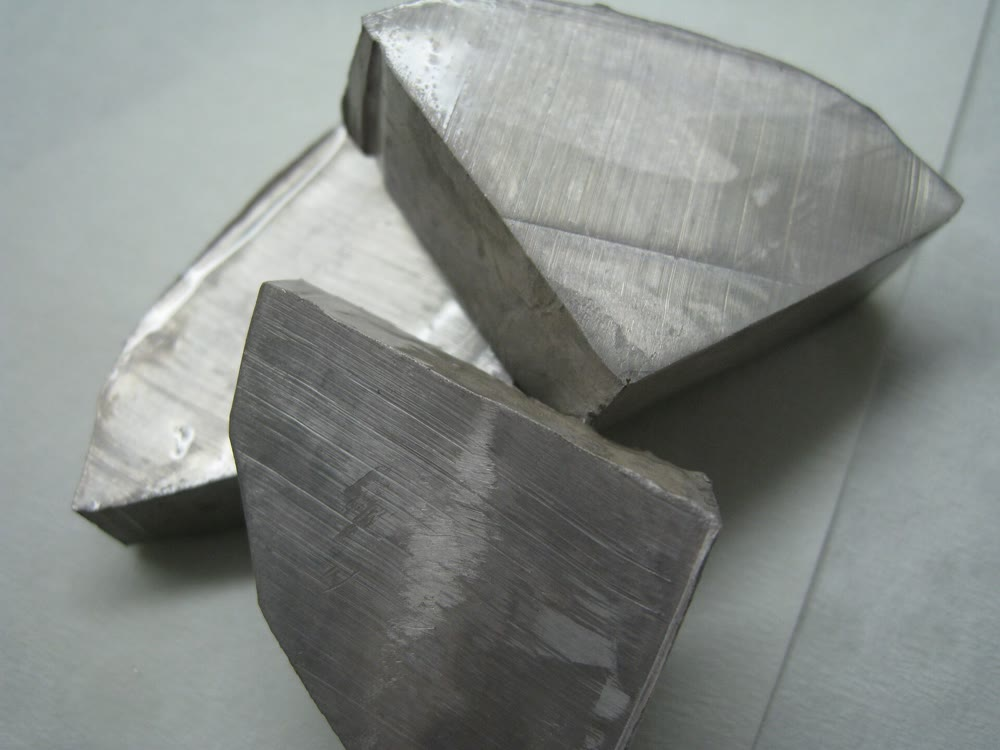
\includegraphics[width=\linewidth,height=4.4cm,keepaspectratio]{images/book1/sodium.jpg}

{\small सोडियम, एक \omterm{def:g10:electron-shells:family}{क्षार धातु}, चाकू से कटा हुआ: ताज़ा होने पर नरम और चाँदी
जैसा, \omterm{def:g4:air-a-mixture-of-gases:air}{वायु} में तुरंत धुँधला पड़ जाता है। फ़ोटो: डीएनएन87, CC BY-SA 3.0।}
\end{minipage}\hfill
\begin{minipage}[b]{0.48\linewidth}\centering
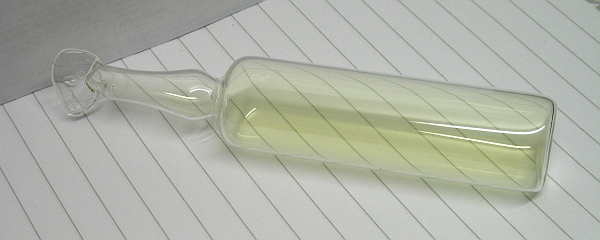
\includegraphics[width=\linewidth,height=4.4cm,keepaspectratio]{images/book1/chlorine-ampoule.jpg}

{\small क्लोरीन, एक \omterm{def:g10:electron-shells:family}{हैलोजन}: पीली-हरी गैस, यहाँ काँच के एक
एम्प्यूल में बंद। फ़ोटो: डब्ल्यू.~ओलेन, CC BY-SA 3.0।}
\end{minipage}
\end{omfigure}

\begin{inthelab}[पानी में सोडियम]
एक पर्दे के पीछे शिक्षक चावल के दाने जितना सोडियम का एक टुकड़ा पानी से भरे बड़े
कटोरे में डालते हैं। वह तैरता है, पिघलकर एक चमकीली गोली बन जाता है और सनसनाता
हुआ इधर-उधर दौड़ता है, जब तक ख़त्म न हो जाए; निकलने वाली गैस हाइड्रोजन है,
और बचा हुआ पानी क्षारकीय है।
\end{inthelab}

\begin{safety}{\ghs[0.75cm]{GHS02}\ghs[0.75cm]{GHS05}\quad\ghs[0.75cm]{GHS03}\ghs[0.75cm]{GHS06}}
% ledger: ghs:Na, ghs:Cl2
सोडियम: पानी के साथ ज्वलनशील हाइड्रोजन छोड़ता है (GHS02), गंभीर रूप से
जलाता है (GHS05)। क्लोरीन: एक ऑक्सीकारक गैस (GHS03), साँस में लेने पर विषैली
(GHS06), साथ ही उत्तेजक और जलीय जीवों के लिए अत्यंत विषैली। दोनों को केवल
शिक्षक ही सँभालते हैं।
\end{safety}

\section{स्थायी आयन और उत्कृष्ट गैस नियम}

\begin{definition}[द्विक और अष्टक नियम]\label{def:g10:electron-shells:octet}
\omterm{def:g10:electron-shells:family}{उत्कृष्ट गैसें}, जिनका बाहरी \omterm{def:g10:electron-shells:configuration}{कोश} भरा होता है, लगभग अभिक्रिया नहीं करतीं: उनका
विन्यास विशेष रूप से स्थायी है। जब पहले तत्वों के \omterm{def:g7:atoms-and-molecules:atom}{परमाणु} \omterm{def:g9:ions:ion}{आयन} बनाते हैं, तो वे
इतने \omterm{def:g9:inside-the-atom:nucleus}{इलेक्ट्रॉन} लेते या खोते हैं कि निकटतम \omterm{def:g10:electron-shells:family}{उत्कृष्ट गैस} का विन्यास पा लें:
सबसे हल्के \omterm{def:g7:atoms-and-molecules:atom}{परमाणुओं} के लिए हीलियम की तरह \omterm{def:g10:electron-shells:configuration}{कोश} 1 में दो \omterm{def:g9:inside-the-atom:nucleus}{इलेक्ट्रॉन} --- यह
\emph{द्विक नियम}\index{द्विक नियम} है --- और बाकी के लिए नियॉन या आर्गन की
तरह बाहरी \omterm{def:g10:electron-shells:configuration}{कोश} में आठ \omterm{def:g9:inside-the-atom:nucleus}{इलेक्ट्रॉन} --- यह
\emph{अष्टक नियम}\index{अष्टक नियम} है।
\end{definition}

\begin{example}[नियम से अनुमानित आयन]\label{ex:g10:electron-shells:ions}
सोडियम, $2.8.1$, अपना अकेला \omterm{def:g10:electron-shells:valence}{संयोजकता इलेक्ट्रॉन} खोता है: \ce{Na+}, $2.8$, नियॉन
जैसा। मैग्नीशियम, $2.8.2$, दो खोता है: \ce{Mg^{2+}}। ऐलुमिनियम, $2.8.3$,
तीन खोता है: \ce{Al^{3+}}। क्लोरीन, $2.8.7$, एक लेता है: \ce{Cl-}, $2.8.8$,
आर्गन जैसा। ऑक्सीजन, $2.6$, दो लेती है: \ce{O^{2-}}। सल्फ़र, $2.8.6$:
\ce{S^{2-}}। लिथियम, $2.1$, एक खोता है और हीलियम की तरह $2$ रखता है:
\ce{Li+}।
\end{example}

\begin{omfigure}
\begin{tikzpicture}[font=\small]
  \foreach \x/\nm/\cfg/\col in {0/{Na}/{$1\mathrm{s}^2\,2\mathrm{s}^2\,2\mathrm{p}^6\,3\mathrm{s}^1$}/omDef,
      5.8/{\ce{Na+}}/{$1\mathrm{s}^2\,2\mathrm{s}^2\,2\mathrm{p}^6$}/omProp,
      11.0/{Ne}/{$1\mathrm{s}^2\,2\mathrm{s}^2\,2\mathrm{p}^6$}/gray} {
    \node[draw=\col, fill=\col!6, rounded corners=2pt, align=center, text width=3.4cm]
      at (\x,0) {\textbf{\nm}\\ \cfg};
  }
  \draw[->, thick, omProp] (2.0,0) -- (3.8,0) node[midway, above, font=\footnotesize] {1 \ce{e-} खोता है};
  \node at (8.4,0) {$=$};
  \node[font=\footnotesize, align=center] at (8.4,-0.75) {एक ही\\ विन्यास};
\end{tikzpicture}

{\small सोडियम \omterm{def:g9:ions:ion}{आयन} का विन्यास निकटतम \omterm{def:g10:electron-shells:family}{उत्कृष्ट गैस}, नियॉन, जैसा
है।}
\end{omfigure}

\begin{remark}[नियम की सीमाएँ]\label{rem:g10:electron-shells:limits}
यह नियम पहले बीस तत्वों और उनके सरल \omterm{def:g9:ions:ion}{आयनों} के लिए अच्छा काम करता है। बहुत-से तत्व,
जैसे लोहा (\ce{Fe^{2+}} और \ce{Fe^{3+}}), इसका पालन नहीं करते; इसके कारण, और
\omterm{def:g9:inside-the-atom:nucleus}{इलेक्ट्रॉनों} का बेहतर वर्णन, विश्वविद्यालय के प्रथम वर्ष के खंड में
दिए गए हैं।
\end{remark}

\section{अभ्यास}

\begin{exercise}[$\star$]\label{exo:g10:electron-shells:1}
कार्बन ($Z = 6$), नाइट्रोजन ($Z = 7$) और मैग्नीशियम ($Z = 12$) के \omterm{def:g10:electron-shells:configuration}{इलेक्ट्रॉनिक
विन्यास} लिखिए।
\end{exercise}

\begin{exercise}[$\star$]\label{exo:g10:electron-shells:2}
कार्बन, नाइट्रोजन और मैग्नीशियम में कितने \omterm{def:g10:electron-shells:valence}{संयोजकता इलेक्ट्रॉन} हैं?
\end{exercise}

\begin{exercise}[$\star$]\label{exo:g10:electron-shells:3}
विन्यास
$1\mathrm{s}^2\,2\mathrm{s}^2\,2\mathrm{p}^6\,3\mathrm{s}^2\,3\mathrm{p}^3$ वाला तत्व किस \omterm{def:g9:periodic-table-first-look:period}{आवर्त} और किस समूह में है?
\end{exercise}

\begin{exercise}[$\star$]\label{exo:g10:electron-shells:4}
इस अध्याय के तीनों परिवारों के नाम बताइए और हर एक के दो तत्व बताइए।
\end{exercise}

\begin{exercise}[$\star$]\label{exo:g10:electron-shells:5}
\omterm{def:g10:electron-shells:octet}{अष्टक नियम} बताइए।
\end{exercise}

\begin{exercise}[$\star\star$]\label{exo:g10:electron-shells:6}
\omterm{def:g10:electron-shells:family}{उत्कृष्ट गैस} नियम की मदद से पोटैशियम ($Z = 19$) और फ़्लुओरीन ($Z = 9$) द्वारा
बनने वाले \omterm{def:g9:ions:ion}{आयन}, उनके विन्यासों के साथ, बताइए।
\end{exercise}

\begin{exercise}[$\star\star$]\label{exo:g10:electron-shells:7}
एक तत्व के तीसरे \omterm{def:g10:electron-shells:configuration}{कोश} में 2 \omterm{def:g9:inside-the-atom:nucleus}{इलेक्ट्रॉन} हैं और तीसरा \omterm{def:g10:electron-shells:configuration}{कोश} ही उसका बाहरी
\omterm{def:g10:electron-shells:configuration}{कोश} है। उसका विन्यास, \omterm{def:g9:inside-the-atom:atomic-number}{परमाणु क्रमांक} और नाम बताइए।
\end{exercise}

\begin{exercise}[$\star\star$]\label{exo:g10:electron-shells:8}
स्थायी \omterm{def:g9:ions:ion}{आयनों} की मदद से मैग्नीशियम और क्लोरीन द्वारा, फिर ऐलुमिनियम और ऑक्सीजन
द्वारा बनने वाले \omterm{def:g9:ions:ionic-compound}{आयनिक यौगिक} का सूत्र लिखिए।
\end{exercise}

\begin{exercise}[$\star\star$]\label{exo:g10:electron-shells:9}
पहले बीस तत्वों की सारणी देखिए। किन तत्वों में ऑक्सीजन जितने
\omterm{def:g10:electron-shells:valence}{संयोजकता इलेक्ट्रॉन} हैं?
\end{exercise}

\begin{exercise}[$\star\star$]\label{exo:g10:electron-shells:10}
सोडियम और क्लोरीन के विपरीत, नियॉन \omterm{def:g7:chemical-reactions:reaction}{रासायनिक अभिक्रियाओं} में कोई \omterm{def:g9:ions:ion}{आयन} क्यों
नहीं बनाती?
\end{exercise}

\begin{exercise}[$\star\star$]\label{exo:g10:electron-shells:11}
\omterm{def:g9:ions:ion}{आयन} \ce{X^{2+}} का विन्यास आर्गन जैसा है। $X$ ज्ञात कीजिए।
\end{exercise}

\begin{exercise}[$\star\star\star$]\label{exo:g10:electron-shells:12}
हीलियम में 2 \omterm{def:g10:electron-shells:valence}{संयोजकता इलेक्ट्रॉन} हैं, फिर भी वह \omterm{def:g9:periodic-table-first-look:period}{समूह} 2 में नहीं, \omterm{def:g9:periodic-table-first-look:period}{समूह} 18 में है।
उसके विन्यास की मदद से समझाइए।
\end{exercise}

\begin{exercise}[$\star\star\star$]\label{exo:g10:electron-shells:13}
पोटैशियम सोडियम से भी अधिक तीव्रता से पानी के साथ अभिक्रिया करता है। \omterm{def:g10:electron-shells:valence}{संयोजकता
इलेक्ट्रॉन} की \omterm{def:g9:inside-the-atom:nucleus}{नाभिक} से दूरी के आधार पर कारण सुझाइए।
\end{exercise}

\begin{exercise}[$\star\star\star$]\label{exo:g10:electron-shells:14}
\ce{S^{2-}}, \ce{Cl-}, \ce{K+} और
\ce{Ca^{2+}} के विन्यास बताइए। इनमें क्या समान है?
\end{exercise}

\begin{exercise}[$\star\star\star$]\label{exo:g10:electron-shells:15}
\omterm{def:g9:periodic-table-first-look:period}{आवर्त} 3 का एक तत्व \omterm{def:g9:ions:ion}{आयन} \ce{Y^{3-}} बनाता है। उसका समूह, उसका
विन्यास और उसका नाम ज्ञात कीजिए।
\end{exercise}

\section{समस्या: माणिक्य, नीलम और कुरुंड}

\begin{problem}[{सप्ताहांत समस्या --- एक रत्न के पीछे के इलेक्ट्रॉन: दो विन्यासों से
एक ग्राम में स्थानांतरित इलेक्ट्रॉनों की संख्या तक}]
\label{pb:g10:electron-shells:1}
माणिक्य और नीलम कुरुंड के रत्न-रूप हैं, जो ऐलुमिनियम और ऑक्सीजन का एक \omterm{def:g9:ions:ionic-compound}{आयनिक
यौगिक} है; दूसरी \omterm{def:g9:periodic-table-first-look:metal}{धातुओं} की सूक्ष्म मात्रा उन्हें उनके रंग देती है।
कुरुंड इतना कठोर है कि लगभग हर चीज़ को खरोंच सकता है, और कुरुंड का चूर्ण
लेंसों को चमकाने में काम आता है। एक \omterm{def:g9:inside-the-atom:proton}{न्यूक्लिऑन} का द्रव्यमान
\qty{1.67e-27}{kg} लीजिए; ऐलुमिनियम-27 में 27 \omterm{def:g9:inside-the-atom:proton}{न्यूक्लिऑन} हैं, ऑक्सीजन-16 में 16।

\medskip
\noindent\textbf{भाग I --- \omterm{def:g7:atoms-and-molecules:atom}{परमाणु}।}
\begin{enumerate}
  \item ऐलुमिनियम \omterm{def:g7:atoms-and-molecules:atom}{परमाणु} ($Z = 13$) और ऑक्सीजन \omterm{def:g7:atoms-and-molecules:atom}{परमाणु} ($Z = 8$) के \omterm{def:g9:inside-the-atom:proton}{प्रोटॉनों} और
        \omterm{def:g9:inside-the-atom:nucleus}{इलेक्ट्रॉनों} की संख्या बताइए।
  \item उनके \omterm{def:g10:electron-shells:configuration}{इलेक्ट्रॉनिक विन्यास} लिखिए।
  \item हर एक में कितने \omterm{def:g10:electron-shells:valence}{संयोजकता इलेक्ट्रॉन} हैं? हर एक किस \omterm{def:g9:periodic-table-first-look:period}{आवर्त} और किस
        समूह में है?
  \item ऐलुमिनियम \omterm{def:g9:periodic-table-first-look:metal}{धातु} है या \omterm{def:g9:periodic-table-first-look:metal}{अधातु}? और ऑक्सीजन?
\end{enumerate}

\medskip
\noindent\textbf{भाग II --- \omterm{def:g9:ions:ion}{आयन}।}
\begin{enumerate}[resume]
  \item \omterm{def:g10:electron-shells:octet}{अष्टक नियम} के अनुसार ऐलुमिनियम कौन-सा \omterm{def:g9:ions:ion}{आयन} बनाता है? उसका
        विन्यास लिखिए।
  \item ऑक्सीजन कौन-सा \omterm{def:g9:ions:ion}{आयन} बनाती है? उसका विन्यास लिखिए।
  \item किस \omterm{def:g10:electron-shells:family}{उत्कृष्ट गैस} का विन्यास दोनों \omterm{def:g9:ions:ion}{आयनों} जैसा है?
  \item ऐलुमिनियम \omterm{def:g7:atoms-and-molecules:atom}{परमाणु} कितने \omterm{def:g9:inside-the-atom:nucleus}{इलेक्ट्रॉन} खोता है, और ऑक्सीजन \omterm{def:g7:atoms-and-molecules:atom}{परमाणु} कितने
        लेता है?
\end{enumerate}

\medskip
\noindent\textbf{भाग III --- सूत्र।}
\begin{enumerate}[resume]
  \item इन \omterm{def:g9:ions:ion}{आयनों} के उदासीन यौगिक, कुरुंड, का सूत्र ज्ञात कीजिए।
  \item एक सूत्र-इकाई में ऐलुमिनियम \omterm{def:g7:atoms-and-molecules:atom}{परमाणु} कितने \omterm{def:g9:inside-the-atom:nucleus}{इलेक्ट्रॉन} खोते हैं? ऑक्सीजन
        \omterm{def:g7:atoms-and-molecules:atom}{परमाणु} कितने लेते हैं?
  \item ये दोनों संख्याएँ बराबर क्यों होनी चाहिए?
  \item एक माणिक्य में क्रोमियम \omterm{def:g9:ions:ion}{आयनों} \ce{Cr^{3+}} की सूक्ष्म मात्रा होती है, जो कुछ
        \ce{Al^{3+}} \omterm{def:g9:ions:ion}{आयनों} की जगह लेती है। \ce{Cr^{3+}} \omterm{def:g9:ions:ion}{आयन} आवेशों को बिगाड़े बिना
        \ce{Al^{3+}} \omterm{def:g9:ions:ion}{आयन} की जगह क्यों ले सकता है?
\end{enumerate}

\medskip
\noindent\textbf{भाग IV --- एक ग्राम कुरुंड।}
\begin{enumerate}[resume]
  \item कुरुंड की एक सूत्र-इकाई में कितने \omterm{def:g9:inside-the-atom:proton}{न्यूक्लिऑन} हैं?
  \item एक सूत्र-इकाई का द्रव्यमान निकालिए (\omterm{def:g9:inside-the-atom:nucleus}{इलेक्ट्रॉन} नगण्य)।
  \item \qty{1}{g} कुरुंड में कितनी सूत्र-इकाइयाँ हैं?
  \item यह कितने \ce{Al^{3+}} \omterm{def:g9:ions:ion}{आयन} और \ce{O^{2-}} \omterm{def:g9:ions:ion}{आयन} हैं?
  \item प्रश्न 14 में \omterm{def:g9:inside-the-atom:nucleus}{इलेक्ट्रॉनों} को नगण्य क्यों माना जा सकता है?
  \item \qty{1}{g} कुरुंड बनाने के लिए ऐलुमिनियम से ऑक्सीजन में कितने \omterm{def:g9:inside-the-atom:nucleus}{इलेक्ट्रॉन}
        स्थानांतरित हुए?
\end{enumerate}
\end{problem}
